%------------------------------------------------------------------------------%

\stopcounter
\begin{frame}{Origem}
  O \textbf{Angular Freeze-Tag Problem} surge como um problema de \textbf{\emph{broadcast}} entre satélites em 2018~\cite{Fe18}:
  \bigbreak
  \begin{minipage}{\linewidth}
    \centering
    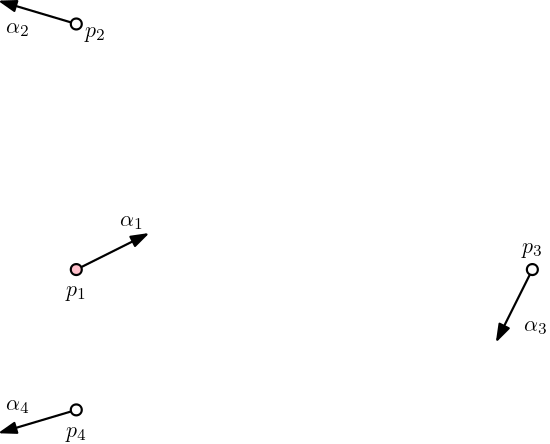
\includegraphics[height=4cm]{AFTP/instance/Temp-0.png}
  \end{minipage}
\end{frame}
\inccounter

\begin{frame}{Motivação}
  \begin{itemize}[<+->]
    \item Dado o crescimento das constelações de satélites, precisamos de estrategias de transmissão eficientes;
    
    \item Recursos limitados restringem a movimentação dos satélites;

    \item Grandes distâncias impossibilitam um \emph{broadcast} simultâneo.
  \end{itemize}
\end{frame}

\begin{frame}{Instância}
  \begin{itemize}[<+->]
    \item Assumimos um \textbf{enxame uniforme};

    \item Conjunto $P = \{p_1, \dots, p_n\}\subseteq \R^2$ de \textbf{posições distintas};

    \item Cada $p_i$ está associado a um satélite com \textbf{ângulo inicial} $\alpha_i$;

    \item Inicialmente, apenas $p_1$ contém \textbf{um dado} a ser propagado;

    \item Apenas os satélites que já receberam o dado podem ajustar suas antenas.
  \end{itemize}
\end{frame}

\begin{frame}{Solução}
  \centering
  \textbf{Rotações} a serem seguidas \textbf{após o recebimento} do dado:

  \pause

  \bigskip
  \begin{minipage}{\linewidth}
    \centering
    \colorbox{white}{\multiinclude[format=png, start=0, end=3, graphics={height=5.5cm}]{AFTP/instance/Temp}}
  \end{minipage}
\end{frame}

\begin{frame}{Definição mais Formal}
  \begin{itemize}[<+->]
    \item \textbf{Conjunto de cronogramas} $S$;

    \item O cronograma de cada satélite $p_i\in P$ é composto por uma \textbf{direção inicial} $d_i$ \pause e uma \textbf{sequência de ângulos} $S_i=(s_{i,1}, \dots, s_{i,k_i})$.
  \end{itemize}
\end{frame}

\begin{frame}{Exemplo}
  \begin{minipage}{\linewidth}
    \centering
    \colorbox{white}{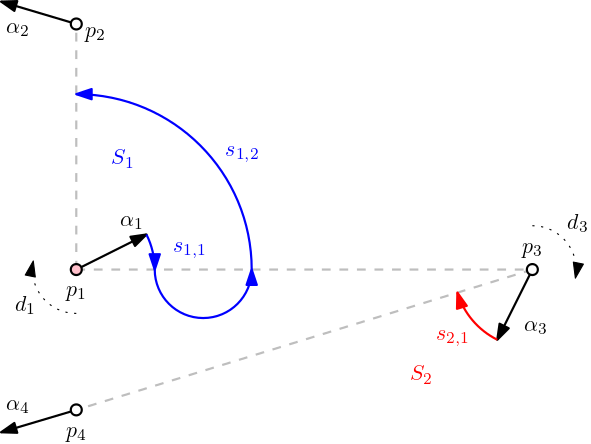
\includegraphics[height=5.5cm]{AFTP/solution.png}}
  \end{minipage}
\end{frame}

\begin{frame}{Dois Objetivos}
  \begin{itemize}[<+->]
    \item O \textbf{makespan ($\mathbf{M(S)}$)} de uma solução $\mathbf{S}$ é o instante em que o último satélite recebe o dado (\textbf{AFTP});
    
    \item A \textbf{energia total ($\mathbf{E(S)}$)} é a soma de todas as rotações realizadas por todos os agentes (\textbf{E-AFTP});
    \bigbreak

    \item Note que $E(S) \ge M(S)$.
  \end{itemize}
\end{frame}

\begin{frame}{Comparação}
  \centering
  Suponha que $\varepsilon < \theta$:

  \bigskip
  \begin{minipage}{\linewidth}
    \centering
    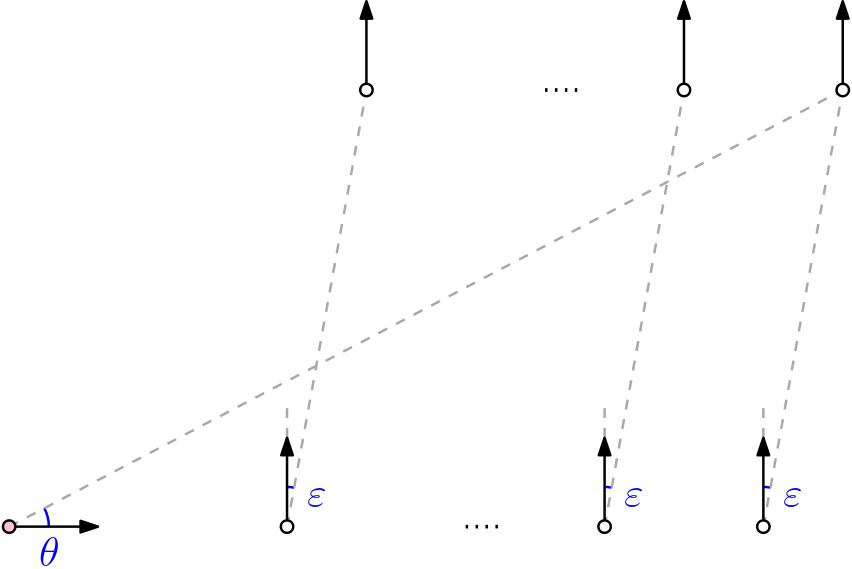
\includegraphics[height=5cm]{AFTP/makespan.png}
  \end{minipage}

  \bigbreak
  \only<2,3>{Seja $\mathbf{S}$ uma solução tal que $\mathbf{M}$ \textbf{é minimizada}.}
  \bigbreak
  \only<3>{Então, $M(S) = \varepsilon$ e $E(S) = \frac{n-1}{2} \cdot \varepsilon = O(n \cdot M(S))$.}
\end{frame}

%------------------------------------------------------------------------------%

\begin{frame}{Resultados Anteriores}
  \begin{thm}[Fekete e Krupke~\cite{Fe18}]
    Existe uma $9$-aproximação para o AFTP em 2D, assumindo um limite inferior de $\delta>0$ para a rotação inicial de qualquer satélite que mova sua antena.
  \end{thm}

  \pause
  \setbeamercolor{block body}{bg=red!20!white}
  \begin{thm}[Fekete e Krupke~\cite{Fe18}]
    É NP-difícil aproximar o AFTP em 2D dentro de um fator menor que $\nicefrac{5}{3}$.
  \end{thm}
\end{frame}
